\documentclass[preprint,11pt]{elsarticle}
\journal{Journal of Biomechanics}
\usepackage{fullpage}
\usepackage[justification=justified,singlelinecheck=false]{caption}
\pagestyle {empty}
\usepackage{amsmath}
\usepackage{tablefootnote}
\usepackage{setspace}
\usepackage{soul}
\usepackage[table]{xcolor}
\bibliographystyle{model5-names}\biboptions{authoryear}
\usepackage[hyphens]{url}
\usepackage{array}
\usepackage{lineno} 




\title{Inter- vs. intra-cycle detrending in the analysis of cyclical biomechanical time series}
%\date{2017\\ December}
\author[1]{Todd C. Pataky}
\author[2]{Guillaume Rao}
\address[1]{\footnotesize Department of Human Health Sciences, Kyoto University, Japan}
\address[2]{\footnotesize Facult\'e des Sciences du Sport, Institut des Sciences du Mouvement,  Aix-Marseille Universit\'e, Marseille, France}









\linenumbers
\begin{document}




%%%%%%%%%%%%%%%%%%%%%%%%%%%%%%%%%%%%%%%%%%%%%%%%%%%%%%%%%%
%%%
% ABSTRACT
%%%
\begin{abstract}
(in preparation) 





\end{abstract}
\maketitle

\vspace{10mm}

Word counts:

Abstract:   xxx  (max 250)

Main text:   xxxx  (max 2000)

\vspace{10mm}



\vspace{10mm}
Corresponding Author:

Todd Pataky, pataky.todd.2m@kyoto-u.ac.jp, +81-075-751-4175





%%%%%%%%%%%%%%%%%%%%%%%%%%%%%%%%%%%%%%%%%%%%%%%%%%%%%%%%%%
%%%
% INTRODUCTION
%%%

\clearpage
\section{Introduction}
\label{sec:introduction}
\doublespacing

(in preparation)




%%%%%%%%%%%%%%%%%%%%%%%%%%%%%%%%%%%%%%%%%%%%%%%%%%%%%%%%%%
% METHODS
%%%
\section{Methods}
\label{sec:methods}

\subsection{Datasets}

One simulated and one experimental dataset were analyzed. The simulated dataset consisted of the \citep{Schwartz2008}

\subsection{Detrending}

aaa

\subsection{Statistics}

Statistical analysis was conducted on only the experimental dataset.








%%%%%%%%%%%%%%%%%%%%%%%%%%%%%%%%%%%%%%%%%%%%%%%%%%%%%%%%%%
% RESULTS
%%%
\section{Results}
\label{sec:results}

aaa


%%%%%%%%%%%%%%%%%%%%%%%%%%%%%%%%%%%%%%%%%%%%%%%%%%%%%%%%%%
% DISCUSSION
%%%
\section{Discussion}
\label{sec:discussion}

(in preparation)




\section*{Acknowledgments}

(in preparation)


\section*{Conflict of Interest Statement}
The authors report no conflict of interest, financial or otherwise.


\bibliography{refs}


\clearpage
\section*{Figures}












\begin{figure}[h]
\begin{center}
	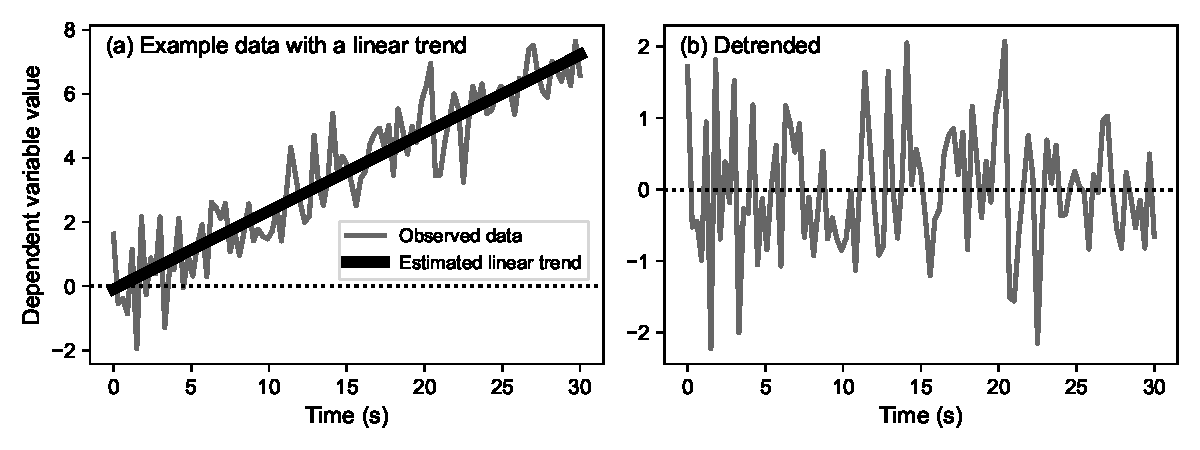
\includegraphics[width=0.99\textwidth]{./figs/fig_common.pdf}\vspace{0mm}
	\caption[Dummy caption.]{Common detrending example.}
	\label{fig:common}
\end{center}
\end{figure}



\begin{figure}[h]
\begin{center}
	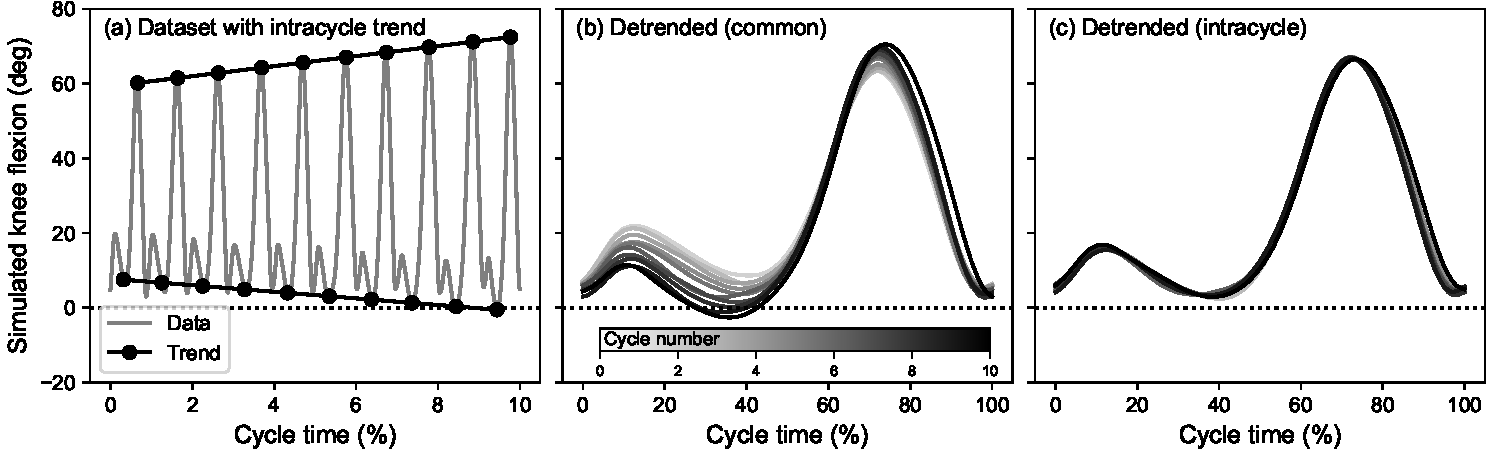
\includegraphics[width=0.99\textwidth]{./figs/fig_intracycle.pdf}\vspace{0mm}
	\caption[Dummy caption.]{Example intracycle trend with detrending results.}
	\label{fig:intracycle}
\end{center}
\end{figure}



\begin{figure}[h]
\begin{center}
	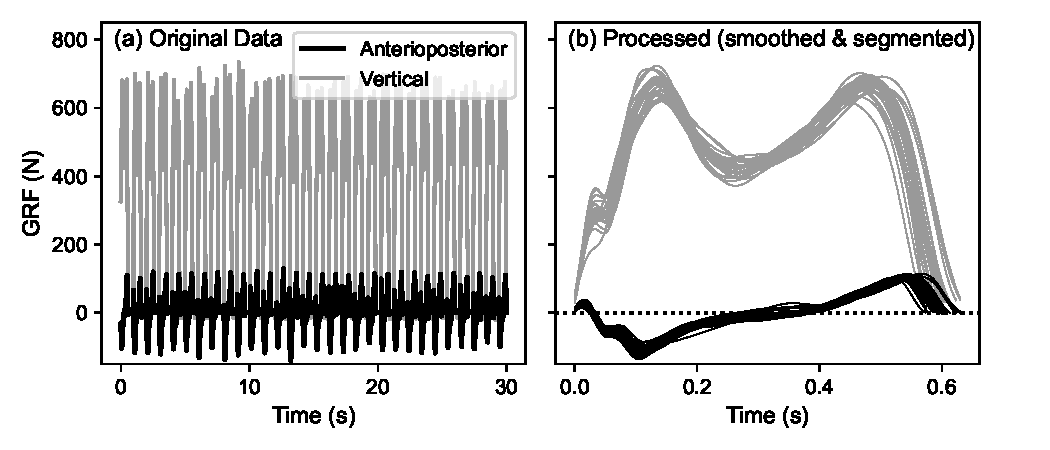
\includegraphics[width=0.99\textwidth]{./figs/fig_grf_dataset.pdf}\vspace{0mm}
	\caption[Dummy caption.]{Experimental dataset from Fukuchi et al. (2018).}
	\label{fig:grf_dataset}
\end{center}
\end{figure}




\begin{figure}[h]
\begin{center}
	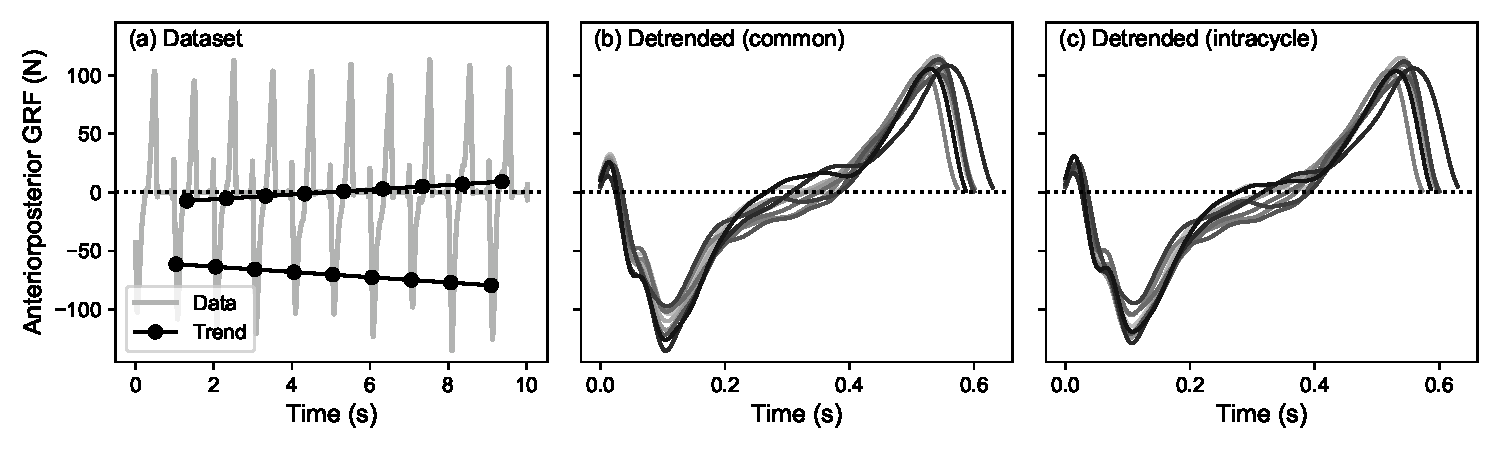
\includegraphics[width=0.99\textwidth]{./figs/fig_results_detrend.pdf}\vspace{0mm}
	\caption[Dummy caption.]{Detrending results for the experimental GRF dataset.}
	\label{fig:results_detrend}
\end{center}
\end{figure}



\begin{figure}[h]
\begin{center}
	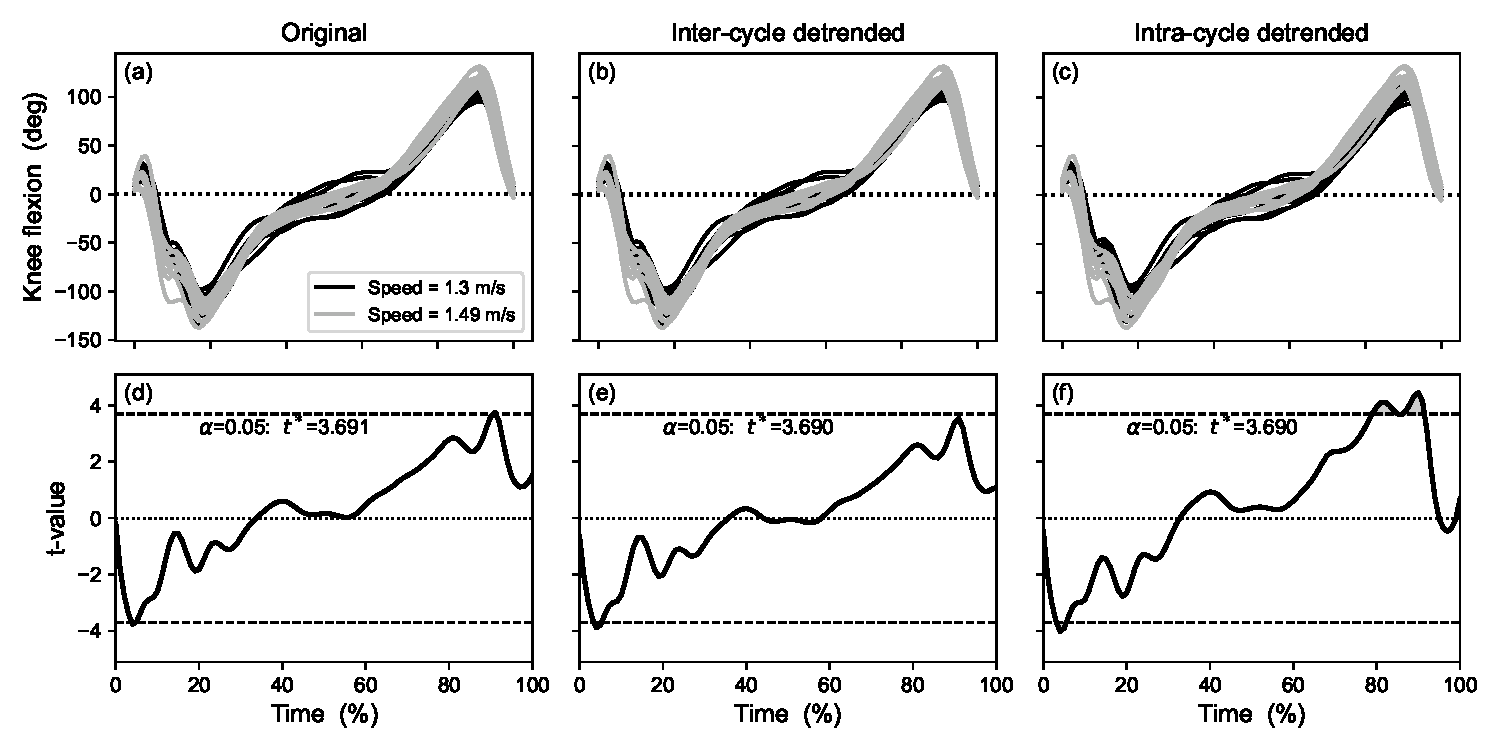
\includegraphics[width=0.99\textwidth]{./figs/fig_spm_01.pdf}\vspace{0mm}
	\caption[Dummy caption.]{Two-sample t-test results for speeds = 1.3 and 1.49 m/s.}
	\label{fig:spm01}
\end{center}
\end{figure}


\begin{figure}[h]
\begin{center}
	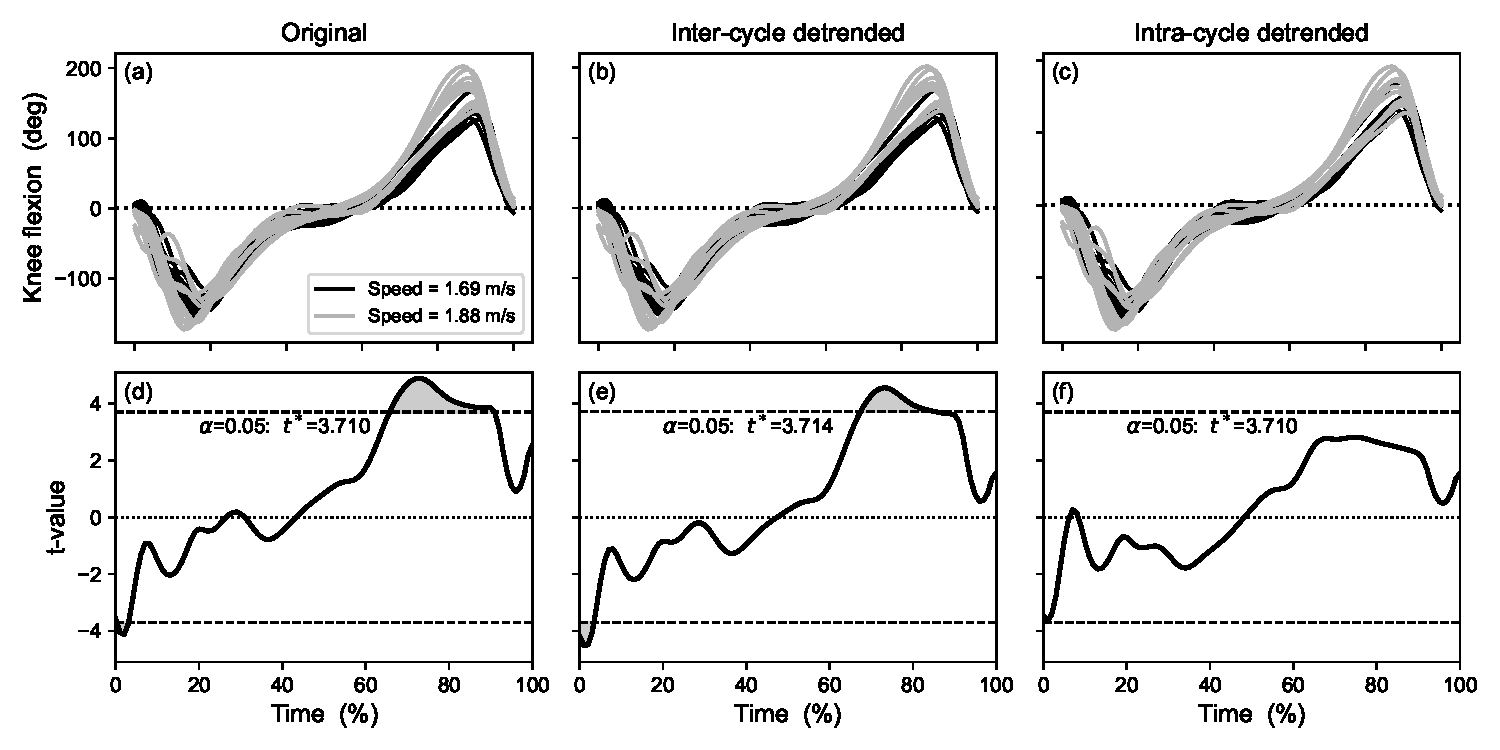
\includegraphics[width=0.99\textwidth]{./figs/fig_spm_23.pdf}\vspace{0mm}
	\caption[Dummy caption.]{Two-sample t-test results for speeds = 1.69 and 1.88 m/s.}
	\label{fig:spm23}
\end{center}
\end{figure}



\end{document}







%\begin{table}[ht]
%\caption{Proposed nomenclature for statistical parametric mapping (SPM) analyses of 1D continua.}
%\begin{tabular}{| p{1.9cm} | p{2cm} | p{1.5cm} | p{9.0cm} |}
%\hline
%Category & Term & Abbreviation & Description\\
%\hline
%\end{tabular}
%\label{table:nomenclature}
%\end{table}

